\section{Développements Logiciel: Conception, Modélisation, Implémentation} 
\subsection{Description des modules utilisés}
% présenter les développements logiciels réalisés dans le cadre du projet
Pour la réalisation de ce projet, nous avons développé un logiciel qui permet de jouer
aux jeux de stratégie combinatoire abstraits du Hex et de l'Awalé avec la Possibilité
d'ajouter facilement d'autres jeux combinatoires et d'appliquer le MinMax dessu. Ce logiciel est
composé de plusieurs modules, dont les principaux sont les suivants:

% présenter les principaux modules du logiciel développé dans le cadre du projet
% Utiliser le langage UML pour la modélisation : donner le diagramme de cas
% d'utilisation et le diagramme des classes
\begin{itemize}
    \item \textbf{Module Hex:} Ce module contient les classes et les fonctions nécessaires
    pour jouer au jeu de Hex. Il contient notamment la classe \texttt{HexBoard} qui 
    représente le plateau de jeu et les joueurs du jeu de Hex. Ce module contient également 
    les fonctions pour l'implémentation de l'algorithme MinMax avec élagage alpha-bêta pour 
    la résolution du jeu de Hex.
    
    \item \textbf{Module Awalé:} Ce module contient les classes et les fonctions nécessaires
    pour jouer au jeu de l'Awalé. Il contient la classe \texttt{AwaleBoard} qui représente le
    plateau de jeu et les joueurs du jeu de l'Awalé. Ce module contient également les fonctions
    pour l'implémentation de l'algorithme de MinMax pour la résolution du jeu de l'Awalé. (a noter que la fonction MinMax
    en elle meme est la meme pour les 2 jeux seule les fonctions d'evalutaions changent.)
    
    \item \textbf{Module Interface Graphique:} Ce module contient les fichiers HTML, CSS et
    JavaScript nécessaires pour l'implémentation de l'interface graphique des jeux de Hex et
    d'Awalé. Il contient notamment les fichiers \texttt{home.html}, \texttt{hex.html} et
    \texttt{awale.html} qui permettent à l'utilisateur de choisir le jeu auquel il veut jouer
    et les paramètres de la partie. Il contient également des fichiers JavaScript pour la
    gestion des événements et des interactions avec l'utilisateur.
    
    \item \textbf{Module Tests:} Ce module contient les fichiers de tests unitaires pour les
    classes et les fonctions des modules Hex et Awalé. Il contient notamment les fichiers
    \texttt{test\_hex.py} et \texttt{test\_awale.py}, qui permettent de tester les classes
    et les fonctions des modules Hex et Awalé.
\end{itemize}


% décrire les fonctionnalités de l'interface graphique implémentée (si votre 
% logiciel dispose d'une interface graphique)
\paragraph{Fonctionnalités de l'interface graphique}
L'interface graphique de notre logiciel comprend une page d'accueil qui permet à l'utilisateur
de choisir le jeu auquel il veut jouer (Hex ou Awalé), une page principale (home) pour chaque jeu
qui permet à l'utilisateur de choisir les paramètres de la partie (taille du plateau (pour Hex),
mode de jeu (joueur contre joueur, joueur contre ordinateur, ordinateur contre ordinateur),
(pour l'ordinateur), etc.) la page home permet aussi de consulter les regles du jeu que nous avons choisi.
Ensuine nous sommes dirigés vrs la page du jeu ou nous pouvons jouer direcement en cliquant sur la page.
Sur les 2 jeu il est possible de previsualiser le prochain coup garce a des fonctions "hover" quand la souris passe
au dessu de cerains elements.
Sur le Hex il est possible de changer le theme graphique de la page avec la touche "H" cela change la page css chargée dans le navigateur.
L'interface graphique est implémentée en HTML, CSS et JavaScript, et
elle communique avec les modules Hex et Awalé via des appels de fonctions JavaScript à des
fonctions Python via des requêtes json et le module Flask.

\begin{figure}[h]
    \centering
    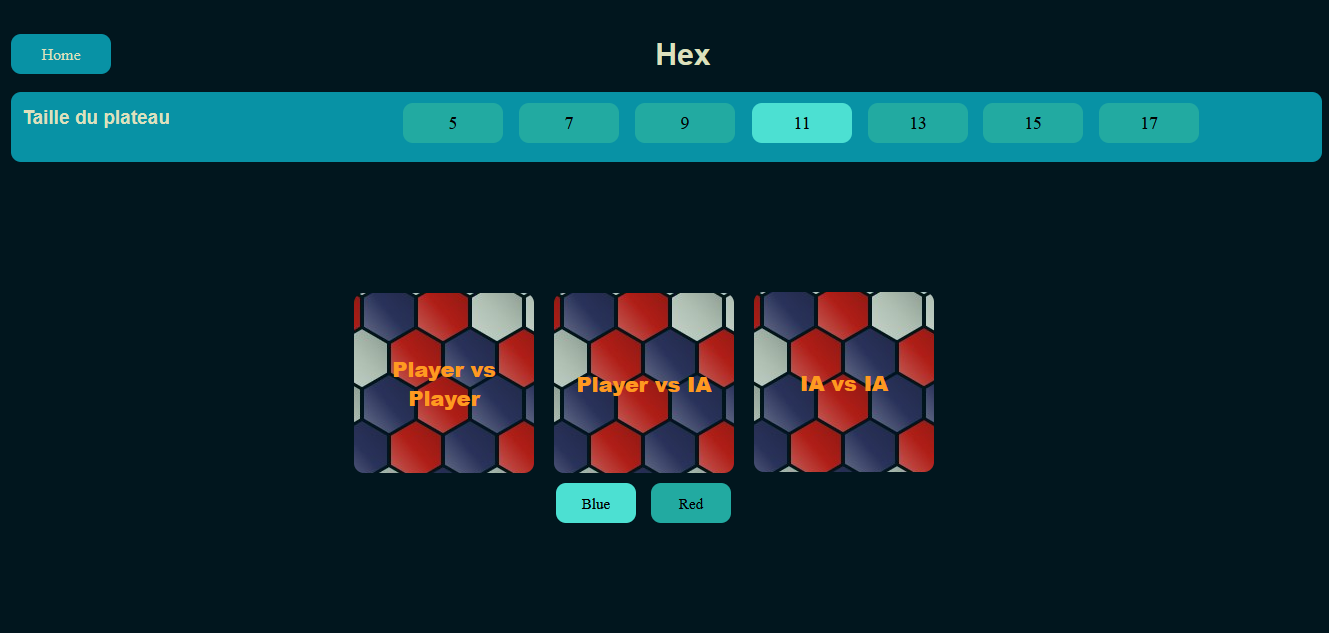
\includegraphics[width=8cm]{root/exemple_home.png}
    \caption{Page Home du Hex}
    \label{fig:exemple_home.png}

    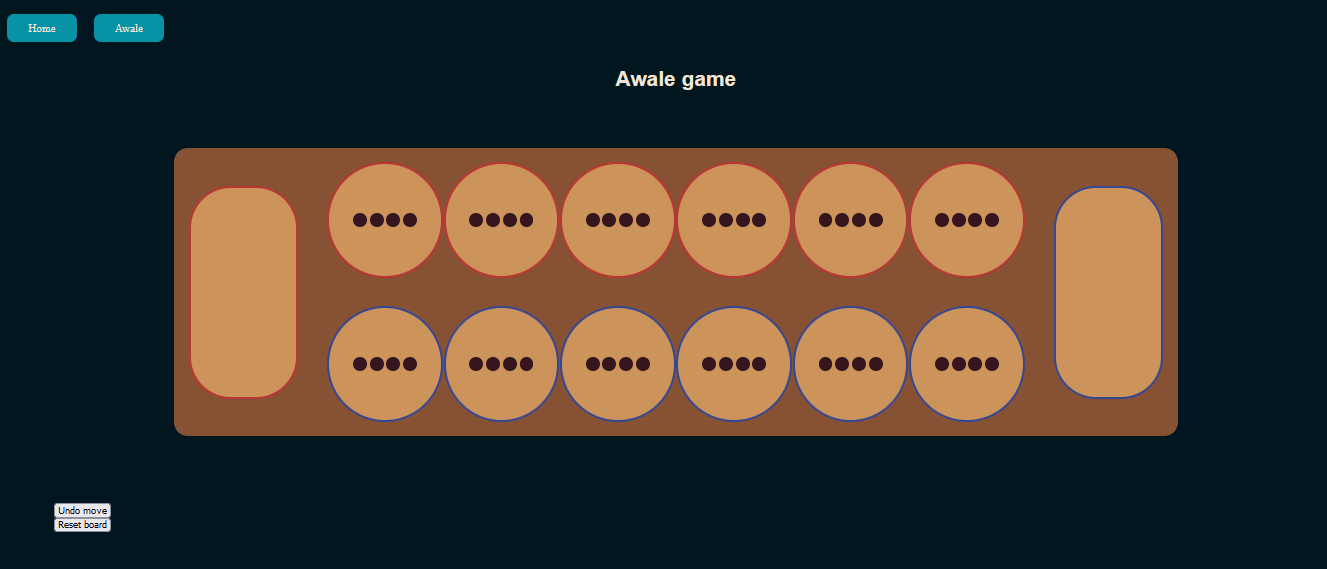
\includegraphics[width=8cm]{root/awale_board.png}
    \caption{Page du jeu Awale}
    \label{fig:awale_board.png}

    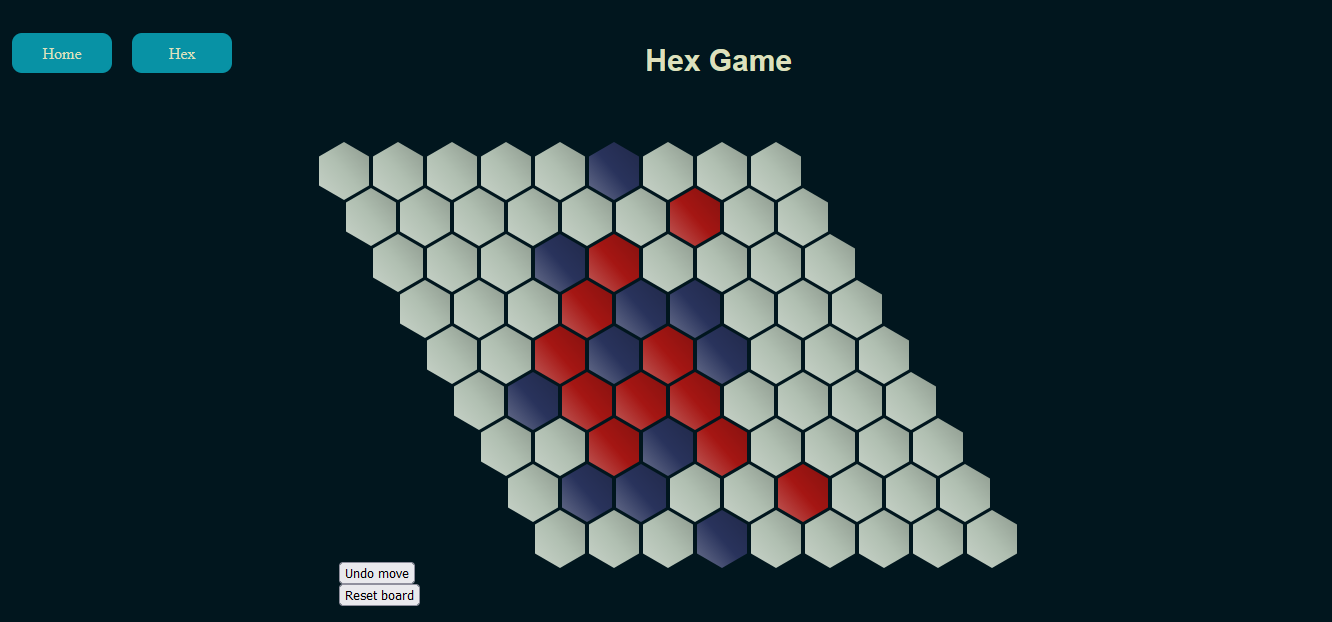
\includegraphics[width=8cm]{root/exemple_partie_hex.png}
    \caption{Page du jeu Hex}
    \label{fig:exemple_partie_hex.png}
\end{figure}

% présenter les principales structures de données définies dans le cadre du
% projet. Décrire le format des données en entrée ou encore les conventions
% utilisées pour les entrées de vos programmes. Décrire les procédures de
% lecture et validation des entrées.
\paragraph{Structures de données}
Les principales structures de données définies dans le cadre de ce projet sont les classes
\texttt{HexBoard} et \texttt{AwaleBoard} qui représentent les plateaux de jeu du Hex et de
l'Awalé, respectivement. Ces classes contiennent les attributs et les méthodes nécessaires
pour représenter les plateaux de jeu et les joueurs, et pour effectuer les opérations de jeu
(placement de pions, déplacement de pions, etc.). Les données en entrée des programmes sont
sous forme de chaînes de caractères qui représentent les paramètres de la partie (taille du
plateau, mode de jeu etc.). Les procédures de lecture et de validation
des entrées sont effectuées par les fonctions des modules Hex et Awalé qui vérifient que les
paramètres de la partie sont valides avant de commencer la partie.

% Statistiques : nombre de modules/composantes/classes/scripts développés.
% Nombre de lignes de code.
\paragraph{Statistiques}
Voici quelques statistiques sur le logiciel développé dans le cadre de ce projet:
\begin{itemize}
    \item Nombre de modules (sans les tests): 39
    \item Nombre de classes : 11 (principalement dans les modules Hex et Awalé)
    \item Nombre de fonctions : 68 (en Python) et 99 (en JavaScript) pour 167 en tout
    \item Nombre de lignes de code : 1 405 (en Python), 2008 (en JavaScript), 553 (en HTML), 1 331 (en CSS)
    et 480 (en \LaTeX) pour un total de 5 777 lignes de code
\end{itemize}

\subsection{Interaction entre fichiers}
% Explication de l'interaction entre les fichiers pendant une partie
Les fichiers de l'application interagissent entre eux de la même façon lors d'une partie de Hex ou 
d'Awalé. Le fichier \texttt{app.py} héberge l'application flask et gère l'interaction entre le frontend et le 
backend pour les 2 jeux.

\paragraph{Initialisation de la partie}
La sélection du jeu et des paramètres de la partie se fait dans le fichier \texttt{home\_hex.html}
(respectivement \texttt{home\_awale.html} pour l'Awalé). Ces informations seront envoyées au fichier \texttt{app.py}
lors de l'appui sur l'un des boutons de lancement de partie. Le bouton sélectionné appellera dans le fichier \texttt{app.py} la 
fonction adéquate renvoyant la page html correspondant aux choix fait par le(s) joueur(s). En parallèle, une instance du plateau de
jeu désiré sera créée dans l'\texttt{app.py}. 

\paragraph{Déroulement d'une partie}
Lorsqu'une partie est jouée, l'information des pièces placées au Hex, ou des graines déplacées à l'Awalé est récupérée par
le fichier JavaScript adapté. Par exemple \texttt{game\_hexia.js} si la partie est une partie de Hex joueur contre l'ordinateur, ou encore 
\texttt{game\_awale.js} si la partie est une partie d'Awalé joueur contre joueur. Cette information est gérée par le capteur d'événements
hex.onclick pour le Hex et pit.onclick pour l'Awalé. Si un tel événement est entendu, le fichier JavaScript correspondant envoie une requête 
json au fichier \texttt{app.py} afin de savoir si le coup est valide. La validité du coup est gérée par une fonction appelée dans la classe du
plateau de jeu adéquat. Si le coup est valide, alors celui-ci est joué et rajouté à l'instance du plateau de jeu. Il est ensuite renvoyé au fichier 
JavaScript qui va s'occuper du nouvel affichage graphique (En modifiant le CSS ou le html). Si une erreur est attrapée, elle est renvoyée
au fichier JavaScript qu'il va gérer en affichant une alerte sur l'écran du joueur indiquant la non-validité du coup. Lors du placement de chaque
hex (déplacement de graines pour l'Awalé), la fonction \textit{check\_winner} de la classe du plateau est appelée afin de vérifier si un joueur à 
gagné. Si c'est le cas, alors la fonction questionnée par la requête json renvoie la variable \textsf{game\_over} égale à \textbf{True}. 
En récupérant cette variable, le fichier JavaScript va pouvoir procéder à une animation indiquant au(x) joueur(s) que la partie est terminée.



\subsection{Fonctions asynchrones}
L'envoie des différentes requêtes des fichiers JavaScript à \texttt{app.py} se fait grâce aux différents appels à la fonction fetch.
La méthode globale \textit{fetch} démarre le chargement d'une ressource sur le réseau et retourne une promesse qui est résolue dès que la 
réponse est disponible. Cependant, le fait que la réponse ne soit renvoyée que lorsque celle-ci est disponible nous a gêné lors de l'implémentation
des modes JcIA et IAvIA pour les deux jeux. En effet, nous souhaitons que notre programme s'exécute de façon synchrone (ligne après ligne). 
Or le \textit{fetch} peut prendre un certain temps avant de résoudre la promesse faite, cela est notamment dû à la lenteur des fonctions d'évaluation.
Ainsi, pour éviter que le reste du programme ne s'exécute avant la résolution de la prommesse, nous avons décidé d'ajouter le décorateur 
\textsf{async} à notre fonction \textit{window.onload}. Ce simple décorateur nous a alors permis d'utiliser le mot-clé \textsf{await}. Celui-ci 
interrompt l'exécution de la fonction asynchrone et attend la résolution de la promesse passée. Ainsi, les requêtes se voient toujours résolues 
avant d'exécuter la suite du programme. Cela permet d'éviter que le joueur joue plusieurs coups pendant que l'IA « réfléchie », ou encore le fait
qu'une des deux IA dans le IAvIA joue plusieurs fois avant que l'autre ne joue.
